% READ FIRST:
% When compiling on TeXmaker, make sure to compile with BibLaTeX (easiest option: change "Quick Build" to compile with: PDFLaTeX + BibLaTeX + PDFLaTeX (2x) + View PDF)

\documentclass[12pt]{article}
\usepackage[utf8]{inputenc}

\usepackage[style=apa,sorting=nty]{biblatex}
\addbibresource{references/bibliography.bib}

%% Including all packages that have been used in past papers.

\usepackage{graphicx}
\usepackage{amssymb}
\usepackage{amsfonts}
\usepackage{amsmath}
%\usepackage{chicago} 
%Chicago is not part of TeXlive 2023, and needs to be manually installed.
\usepackage{geometry}
\usepackage[bottom]{footmisc}
\usepackage{setspace}
\usepackage{caption}
\usepackage{tabularx}
\usepackage{rotating}
\usepackage{lscape}
\usepackage{version}
\usepackage{fancyhdr}
\usepackage{scalefnt}
\usepackage{booktabs}
\usepackage{threeparttable}



\begin{document}

\title{\underline{Rename Me with Title}\thanks{\noindent \underline{Replace Me Acknowledgments}}}

\author{Razvan Vlaicu \and \underline{Coauthors}}

\date{\underline{Replace Me with Date}}

\maketitle

\begin{abstract}
\underline{Enter Abstract}

\bigskip

\noindent \textbf{JEL Classifications:} \underline{Replace me with JEL Codes}.

\noindent \textbf{Keywords:} \underline{ Replace Me with Keywords.}
\end{abstract}

\bigskip \pagebreak


\section{Template Sample}

\underline{Delete Template Sample section (lines 56-89) once ready for writing paper draft.}

\subsection{Figures}

Figures are stored in the "outputs" folder. Do-File should export three formats of each figure and are stored in the following "figures" subfolders:

\begin{itemize}
	\item \textbf{eps} (best for printing)
	\item \textbf{pdf} (best overall format)
	\item \textbf{png} (best for images)
\end{itemize}


Use the following command to import figure to paper: 

\begin{figure}[ht]
\centering
\caption{\underline{Replace Me with Figure Title}}
\label{fig:Replace_Me_with_Ref_Label}
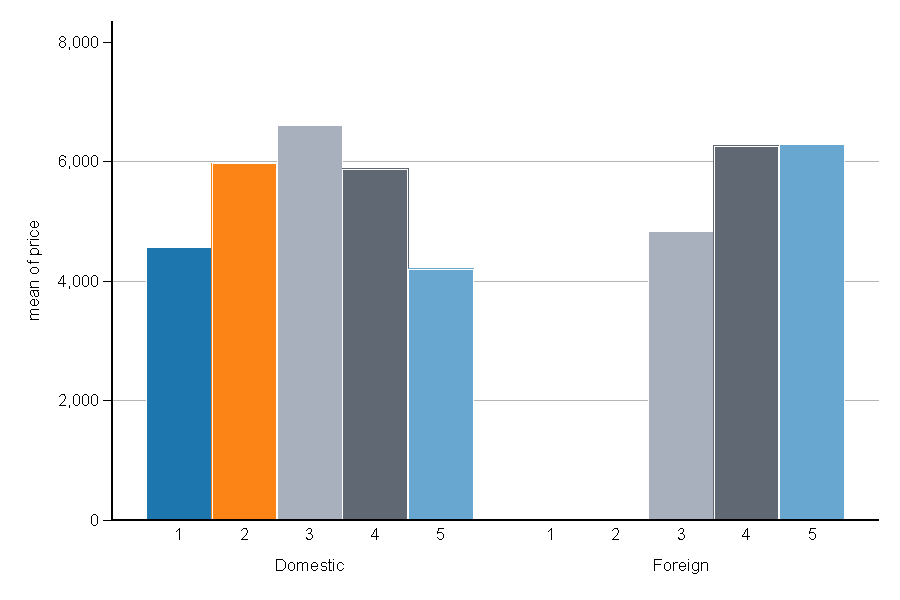
\includegraphics[width=1\textwidth]{outputs/figures/pdf/project_name_figure_name.pdf}
\end{figure}

\subsection{Tables}

Like with Figures, Do-file stores tables in the "tables" subfolder of "outputs." Use the following command to include a table into paper:

\begin{table}[htbp]\centering
\begin{threeparttable}
\caption{Car prices: Domestic vs. Foreign}
\def\sym#1{\ifmmode^{#1}\else\(^{#1}\)\fi}
\begin{tabular} {l*{1}{cc}}
\toprule 
&\multicolumn{2}{c}{}          \\
& Mean & SD                            \\
\midrule
Domestic &  6072.423 &  3097.104\\
Foreign &  6384.682 &  2621.915\\
\bottomrule
\end{tabular}
\begin{tablenotes}[flushleft]
\item Prices in USD. This is a test to see what happens when I write a very lengthy footnote without any breaks. Does it stretch out beyond the table, or does it wrap down to a new row?
\end{tablenotes}
\end{threeparttable}
\end{table}

\subsection{Citations and References}

Citation test \parencite{keefer2022demand}. Figure \ref{fig:Replace_Me_with_Ref_Label} is a pdf version of the MPG graph, meanwhile we can also see this same graph in png format if we change the path name and extension name to "png." This graph displays prices of domestic\footnote{"Domestic" is referring to U.S. made vehicles.\label{fnote:domestic}} 
\& foreign vehicles, by number of repairs.

\section{Introduction}

\underline{Replace Me with Introduction}


\printbibliography 
%% Note, printbibliography creates a non-numbered section, and thus don't need to enter a section command before printing bibliography.

\end{document}